%
% IEEE Transactions on Microwave Theory and Techniques example
% Tibault Reveyrand - http://www.microwave.fr
%
% http://www.microwave.fr/LaTeX.html
% ---------------------------------------



% ================================================
% Please HIGHLIGHT the new inputs such like this :
% Text :
%  \hl{comment}
% Aligned Eq. 
% \begin{shaded}
% \end{shaded}
% ================================================

\documentclass[journal]{IEEEtran}

%\usepackage[retainorgcmds]{IEEEtrantools}
%\usepackage{bibentry}  
\usepackage{xcolor,soul,framed} %,caption

\colorlet{shadecolor}{yellow}
% \usepackage{color,soul}
\usepackage[pdftex]{graphicx}
\graphicspath{{../pdf/}{../jpeg/}}
\DeclareGraphicsExtensions{.pdf,.jpeg,.png}

\usepackage[cmex10]{amsmath}
%Mathabx do not work on ScribTex => Removed
%\usepackage{mathabx}
\usepackage{array}
\usepackage{mdwmath}
\usepackage{mdwtab}
\usepackage{eqparbox}
\usepackage{url}
\usepackage{longtable}

\usepackage{hyperref}
\hypersetup{
    colorlinks=true,
    linkcolor=blue,
    filecolor=magenta,      
    urlcolor=cyan,
}

\hyphenation{op-tical net-works semi-conduc-tor}

%\bstctlcite{IEEE:BSTcontrol}


%=== TITLE & AUTHORS ====================================================================
\begin{document}
\bstctlcite{IEEEexample:BSTcontrol}
    \title{Improve Overall Performace Indicators of The Organization using Data Analysis}
  \author{Dulan~Jayasuriya,~\IEEEmembership{dulan.20@cse.mrt.ac.lk}
      Chanindu~Leelananda,~\IEEEmembership{chanindu.20@cse.mrt.ac.lk}% <-this % stops a space
      \newline
      \\
Department of Computer Science \& Engineering \\

Faculty of Engineering \\
University of Moratuwa \\
Sri Lanka 
% Emails: dulan.20@cse.mrt.ac.lk , chanindu.20@cse.mrt.ac.lk
%   \thanks{This work is a part of MSc in Computer Science specialized in Data science, course modeule CS5617 Data Science project }
%   \thanks{Dr. Uthayasanker Thayasivam (RTU) (e-mail: rtuthaya@cse.mrt.ac.lk).}% <-this % stops a space
%   \thanks{Dr. Shehan Perera (e-mail: erez.falkenstein@gmail.com).}
  }  


% The paper headers
\markboth{Department of Computer Science Engineering Faculty of Engineering University of Moratuwa, April~2020
}{Roberg \MakeLowercase{\textit{et al.}}: High-Efficiency Diode and Transistor Rectifiers}


% ====================================================================
\maketitle

% === ABSTRACT ====================================================================
% =================================================================================
\begin{abstract}
%\boldmath
In a business environment, assuring profitability is a key thing to continuous operation. For the manufacturing industry, maintaining Overall Equipment Efficiency(OEE) is a direct indication of profitability. This project is an initiative to launch Data-driven decision Making(D3M) \cite{provost2013data} in a manufacturing environment. Data Analysis has been carried out in Descriptive, Diagnosis and Predictive along with the visualisations. The main focus of the descriptive analysis was to give a better representation of data and Diagnostic analysis was used to analyze the relationship between different features. The predictive analysis was done using different regression models such as Linear Regression, Support Vector Machines, Decision Trees, Random Forest and Neural Networks in order to identify the best method to predict the outcome from the selected feature points. We were able to explain the relationships between features and achieve 80\% accuracy with the predictive methods. In this approach for data analysis is initiated in a manufacturing environment, it enables the users to visualise the available data in a useful manner in the meantime analyze data and find root causes for efficiency drops. Also by initiating predictive analysis practices, the organisation can get rid of future unfavourable operations in terms of profit.
\end{abstract}

\footnote{Link to the github page. https://github.com/DulanGit/In20-S1-CS5617-project-1}
% === KEYWORDS ====================================================================
% =================================================================================
\begin{IEEEkeywords}
performance indicators, data analysis, business environment, manufacturing industry, overall equipment efficiency 
\end{IEEEkeywords}


% For peer review papers, you can put extra information on the cover
% page as needed:
% \ifCLASSOPTIONpeerreview
% \begin{center} \bfseries EDICS Category: 3-BBND \end{center}
% \fi
%
% For peerreview papers, this IEEEtran command inserts a page break and
% creates the second title. It will be ignored for other modes.
\IEEEpeerreviewmaketitle


% ====================================================================
% ====================================================================
% ====================================================================

% === I. INTRODUCTION =============================================================
% =================================================================================
\section{Introduction}

\IEEEPARstart{T}{he} analysis carried out in this report is based on the operational datasets of an Ice cream manufacturing plant. For this analysis, both production-related data and utility-related data is incorporated. The following paragraph shows a brief company introduction.

The Colombo Ice Company(PVT)Ltd owns an aforesaid factory premise which is a modern Ice cream manufacturing facility that meets world-class standards in terms of both process and equipment. It is located at the Seethawaka export processing zone Awissawellla. This factory consists of 18 utility packages and 8 production Machine packages which facilitates two end product lines for finished goods.

The finished goods of this factory are impulse category Ice cream with volumes less than 100 ml which are in common terms Ice Cream Cups, Sticks(Candy) \& Ice Cream Cones.
There are a number of different products under each category. Giving a brief introduction on  ice cream manufacturing, the first step is to process the ice cream mix, then chocolate and edible cones are manufactured as edible material. Afterwards ice cream mix is pumped into the filling and packing sections in order to produce the desired end product.

In terms of financial perspective, the operation of the factory with a competitive advantage is a key parameter in order to survive in the category of Fast Moving Consumer Goods. There is a severe competition within the Sri Lankan market for frozen confectionery(Ice cream) where approximately 40\% of Impulse Ice cream market share is held by “Elephant House”. Therefore as a business, there are plans to gain more market share. In simpler terms, one of those strategies is by reducing the conversion costs(manufacturing-related cost) by improving efficiencies in terms of all the controllable parameters.

 In a factory environment where production efficiency depends on a number of parameters, it is quite difficult to carry out simple root cause analysis and improve efficiency as it is a simple problem. Now only time-series data is being evaluated weekly basis, how the production quantities and utility consumption with the variation of performance indicators. The issue with this type of illustration is that there are no insights of the day to operations. For example, if OEE of a particular machine has reduced in a day, there is no quantifiable reasoning for the incident. There can be qualitative reasons such as breakdowns have occurred, the material was not delivered on time etc. But there is no indication how much a particular reason affects efficiency. Therefore a systematic approach to analyze the available data set whether it is significant, in order to improve the efficiency of operation.

There are several initiatives launched by operations excellence teams, in Savings projects, Connected factory(IIoT) systems that improve Profitability and Visibility respectively. But proper systematic data analysis initiative with the below-implemented approach will give a next-level competitive advantage for efficiency improvements.

The other important factor which has not yet been exploited in this field is forecasted approach in production planning. i.e. Usually a production plan is an amended version of a demand plan, where the product quantities are dependent on the macro factors. But micro factors such as profitability indicators are not considered due to the fact, those are difficult to predict due to a large number of dependencies at different weights. Therefore in this paper, some predictive data analysis has been done to classify the plan whether it is profitable or not.

Therefore it is an obvious fact that exploring this uncharted area of data science we are able to dig into deeper insights and discover root possibilities to improve efficiencies thus profitability. Also by predictive analysis, there is a possibility to eliminate the inefficient \& production runs which have lower profitability.

Summarising the topic in general concepts, by leading this firm to make better business decisions using analytic methods and create competitive advantages from data then managerial and leadership positions rely on data-driven decision making. Recent studies have shown companies who adopt “Data-Driven Decision Management” achieve significant productivity gains over other firms.



\section{Background}
In the study of data science, we classify the data into different categories to identify the data type. A simple illustration is shown in Fig.~\ref{type_of_features} for different categories of data which some types are being included in this project.

% ==== FIG 1
\begin{figure}
  \begin{center}
  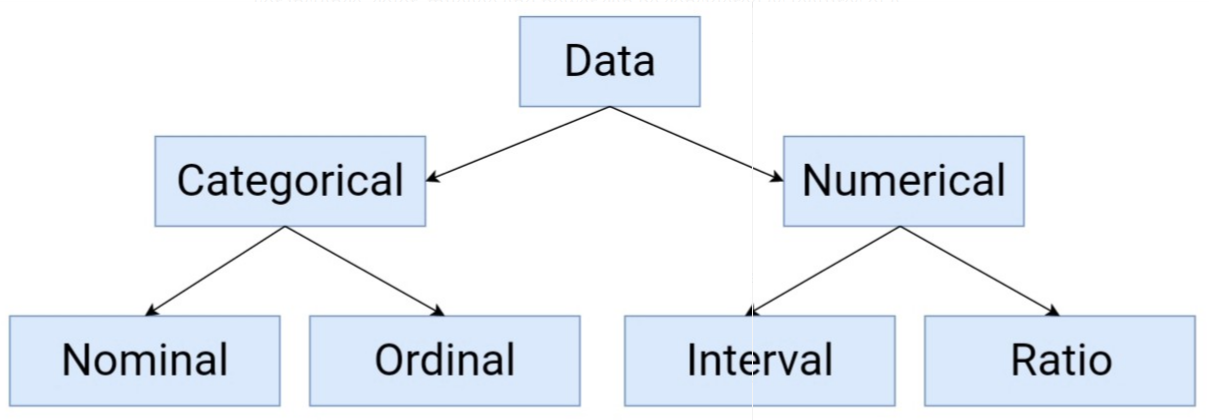
\includegraphics[width=3.2in]{photo/type_of_features.png}
  %\vspace{-15pt}
  \caption{Different data types in statistics.}\label{type_of_features}
  \end{center}
\end{figure}

In this dataset, there are both categorical and numerical data. Giving an introduction to the tables of this data set, in this factory environment, there are two lines which give the end product. Production and performance-related data for those machines are included in separate tables. The other table consists of all the utility data, All the data is captured daily basis over a time period of one year.

The data sources are a set of spreadsheets which is maintained by respective departments in the company. For clarity below table explains the attributes in one of the tables for the production machine, which we have selected to carry out the analysis in the latter part of the project. \\


% =============== Table 1
\begin{center}
\begin{tabular}{ | m{1.5cm} | m{6cm} | } 
\hline
 Attribute Name & Description  \\ 
\hline \hline
Date & The date when operation is carried out  \\ 
 \hline
 Product & The Product that was in manufactured \\ 
 \hline
 Planned Start Time & The time production line was expected to start\\ 
 \hline
 Actual Start Time & The time when that machine actually started \\ 
 \hline
  Stop Time & The time when production of the machine  stopped \\ 
 \hline
  Total Time & Total time spend for production activities including all the delays \\ 
 \hline
 \end{tabular}
 \end{center}
 \begin{center}
 \begin{tabular}{ | m{1.5cm} | m{6cm} | } 
 \hline
 Attribute Name & Description  \\ 
\hline \hline

 Start-up Delay & The delay occurred to start the production line \\
 \hline
  Breakdown delays & Total time wasted for machine breakdowns and other operational delays \\ 
 \hline{}
 Effective prod time & The  time duration which actual production was carried out \\
 \hline
 Operating Speed & Output rate of the machine in eaches:It is number of units per hour \\
 \hline
 Produced Qty & Actual quality approved production quantity in eaches of the product
 \\
 \hline
 Rejects Qty & Quality rejected quantity in eaches of the product \\
 \hline
 Mix Usage & Amount of Ice cream mix(milk) used for filling and packing \\
 \hline
 Mix Wastage & Amount of Ice cream mix wasted prior to filling and packing \\
 \hline
 Mix Yield & Percentage of the mix volume used for production out of total mix volume \\
 \hline
 AR & Percentage: The time machine was ready for production out of total planned time \\
 \hline
 PR & Quality rate Percentage of good products quantity from total  production volume \\
\hline
 QR & Quality rate Percentage of good products quantity from total  production volume \\
\hline
 OEE & Overall equipment efficiency: Product of AR, PR and QR : Overall indicator of the machines  performance \\
\hline
\end{tabular}
\end{center}
% ===============================================

As per the end objectives of this project in order to empower Data-Driven Decision Making(D3M), which is the process of making decisions based on the data rather than mere observations and personal experience, this project is carried out as per the steps of D3M which are, \\

\begin{enumerate}
  \item Store \\
This is how operations data is gathered and stored for an analysis. This part is almost complete since data gathering is completed.
  \item Analyse \\
This is the key component of this project: using the data set, Descriptive, Diagnosis and Predictive analysis is carried out. Under descriptive analysis simple indications have been given on the parameters answering straight questions on the data. Then under-diagnosis analysis detailed indications have been given for several observations based on the dataset. Then in the predictive analysis part based on the past performance, future production has been forecasted and classified to observe whether those are profitable to operate or not.
  \item Visualize \\
After analyzing data, several illustrations has been prepared, such a way that users are able to see through the actual picture and what is really happening. 
  \item Decide \\
Several recommendations has been given based on those visualisations.

\end{enumerate}

% === II. Pre processing section ========================
% =================================================================================
\section{Methodology \& Results}
\subsection {Pre Processing}

Data is often taken from multiple sources which are normally not too reliable and that too in different formats. There may be problems due to human error, limitations of measuring devices, or flaws in the data collection process. Mainly python language \cite{python} and pandas library \cite{pandas} was used to do the data processing. Preprocessing was done as separate stages. \\


\subsubsection {Derive useful features}
Some of the useful indicators can be derived from the existing measurements. Rejects percentage is an example.  These new rows were added to the existing data frame. 
\begin{equation}\label{rejects_percentage}
    Rejects\,Percentage = \frac{Rejects\,Qty}{Produced\,Qty\,+\,Rejects\,Qty}
\end{equation}
\subsubsection {Inconsistent columns}
Dataset itself contains columns that are irrelevant or useless columns that can drop them to give more focus on the other columns that have meaningful information. First, select the columns which are useful for the analysis. There was a lot of redundant data. From the previous experience, the total time has no effect on the efficiency of the product. Also, some columns are highly dependent on others. As an example, the difference between planned start time and the actual start time was directly reflected in the Startup delays. Most useful columns were selected to analyse the data further. \\
\subsubsection {Remove duplicate values (categorical data)}
The product categories were duplicated so some of them had to be renamed to a common name before processing the data. After removing the duplicates the product column unique products were reduced from eighteen to twelve. \\
\subsubsection {Missing Values}
Missing values in a dataset are common in data science. This usually happens in the data collection part or when there is some data validation rule. Regardless of that missing values must be taken into consideration. In this dataset, some of the columns had null values.
There are two common methods to tackle this problem. \\

\begin{itemize}
  \item Estimate missing values \\
  For this dataset some data could be able to be estimated by looking at other columns. 
  \begin{equation}\label{total_time}
    Total\,time = End\,Time - Start\,Time
\end{equation}

Using the above equation null values which appeared in the “Total time” column could be derived from the other columns. 
Some other values were filled by calculating the mean of that specific c
As an example “Mix Yield” column null values are being replaced by the mean of that column.\\


  \item Eliminate the rows with missing values \\
Missing values were found which cannot recover or reconstruct from other features. Some missing data was removed since those data cannot be estimated. \\

\end{itemize}


\subsubsection {Data Normalization}
Data normalization is an important step in most of the analysis problems. Data normalization was done when seeking for relations. Different data were in different ranges, in order to train a regressor, all the data should be normalized. There are different types of data normalization, Z Normalization was used in this study. This transformation sets the mean of the data to 0 and the standard deviation to 1. This was done Feature-wise, for each column. \\

% ==== FIG 2
\begin{figure}[ht]
  \begin{center}
  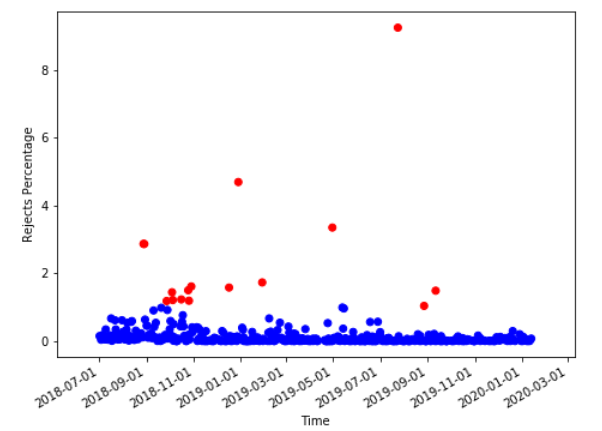
\includegraphics[width=3.2in]{photo/outliers.png}
  %\vspace{-15pt}
  \caption{Identification of Outliers in rejects percentage.}\label{outliers}
  \end{center}
\end{figure}

\subsubsection {One hot encoding}
One hot encoding is a process by which categorical variables are converted into a form that could be provided to ML algorithms to do a better job in prediction. Here a deep neural network was used to predict the data, in order to prepare the data for the input categorized products were converted to one-hot encoding. \\

\subsubsection {Remove the outliers}
In statistics, an outlier is a data point that differs significantly from other observations. That means an outlier indicates a data point that is significantly different from the other data points in the data set. Outliers can be created due to the errors in the experiments or the variability in the measurements.
Some of the values were found in this dataset as abnormal values. Keeping these data will drastically reduce the accuracy of the model. Since some values cannot be estimated by other values, these outliers had to be removed from our dataset. 


For instance Fig.~\ref{outliers}  was plotted the values of rejected percentage. All the values higher than 1 are represented in red colour dots and which are less than 1 represented by blue colour dots. These rows were removed from the dataset in order to clean the dataset. 

% \subsection{Data Analysis}


\subsection {Descriptive Analysis}


A descriptive analysis is an important first step for conducting statistical analyses \cite{jain2000statistical}. Descriptive statistics are used to describe the basic features of the data in a study.  In this section, our main focus is to describe the data gathered during the first phase. Most of the graphs were generated using Seaborn \cite{seaborn} library which is highly focused on visualizations. 

OEE (Overall equipment efficiency) is the main focus of this dataset Since it is the main measurement of the efficiency of this entire production line. A couple of graphs were used to analyse this OEE to check whether how it changes. 

\begin{figure}[ht]
  \begin{center}
  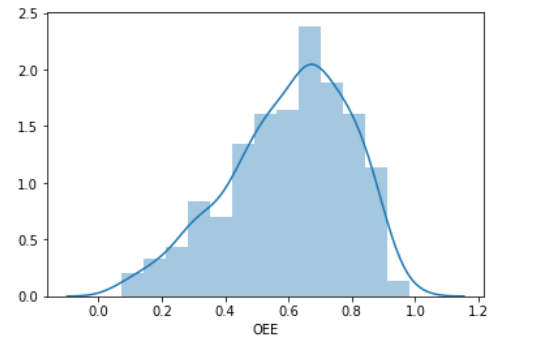
\includegraphics[width=3.2in]{photo/dist_oee.png}
  %\vspace{-15pt}
  \caption{Normal Distribution of OEE}\label{distributionOEE}
  \end{center}
\end{figure}

When checking the distribution of OEE Fig.~\ref{distributionOEE} , it was mainly oscillating around 70\%. Organization's target is to improve this and move this distribution more towards higher percentages. 

\begin{figure}[ht]
  \begin{center}
  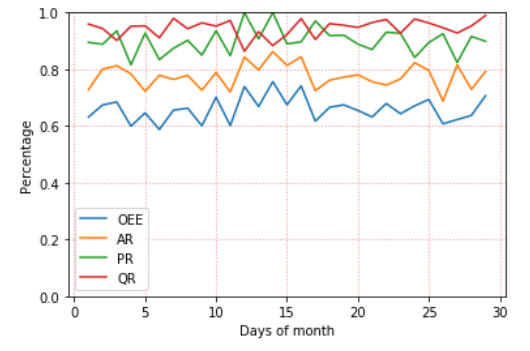
\includegraphics[width=3.2in]{photo/oee_during_month.png}
  %\vspace{-15pt}
  \caption{Daily OEE, AR, PR,QR  variation for a month}\label{OEEMonth}
  \end{center}
\end{figure}

The following Fig.~\ref{OEEMonth} is the OEE(Overall Equipment Efficiency), AR(Availability Rate), PR(Performance Rate), QR(Quality Rate) variation throughout the month.  All these are the final indicators of the efficiency of the production. High efficiencies were observed during the middle of the month (12-17). The reason higher volumes are produced in during the middle of the month in order to cater the sales targets.


\begin{figure}[ht]
  \begin{center}
  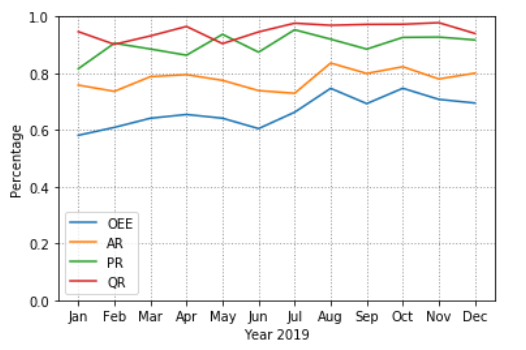
\includegraphics[width=3.2in]{photo/oee_entire_year.png}
  %\vspace{-15pt}
  \caption{Month on Month Average OEE, AR, PR and QR}\label{OEEYear}
  \end{center}
\end{figure}

Another example of descriptive analysis is how the same parameters are shown in Fig.~\ref{OEEYear} graph has a varied month on month during the year 2019. In this graph, it’s clear that the indicators are improving with time. Last year January OEE started around 60\% and it improved to 70\% at the end of 2019. 

\begin{figure}[ht]
  \begin{center}
  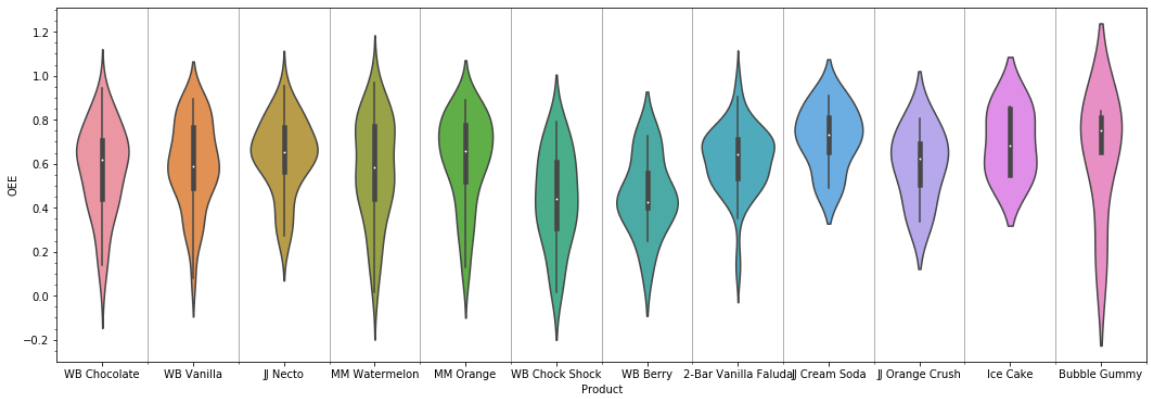
\includegraphics[width=3.3in]{photo/violine.png}
  %\vspace{-15pt}
  \caption{Distribution of OEE product-wise; The highlighted vertically black  component is Q1 Q3 range and white dot indicated the mean. Higher the width of the shape the number of higher the number of occurrences.}\label{ViolineOEE}
  \end{center}
\end{figure}

The visualisation in Fig.~\ref{ViolineOEE} illustrates the variation of OEE for different products manufactured in the stick line. In this violin plot, the white dot represents the mean and the black bar represents the interquartile range. And the entire distribution is represented by the coloured area for each product.  As a descriptive indicator, it is obvious that WB Chock Shock and WB Berry have a lower mean of OEE compared to other products. While Bubble gummy has a wide distribution, Cream soda has the narrowest. We can conclude that Bubble Gummy can be controlled and bring up the OEE, there are some facts that changing with time to time which make it vary the OEE job to job. \\

\subsection {Diagnostic Analysis}

Following Fig.~\ref{OEELastYear} is a sample diagnosis analysis done for the variation of the month on month OEE, reasons for OEE reduction in a particular month is quantifiably analysed. Below figure is the OEE variation for the last year.

\begin{figure}[ht]
  \begin{center}
  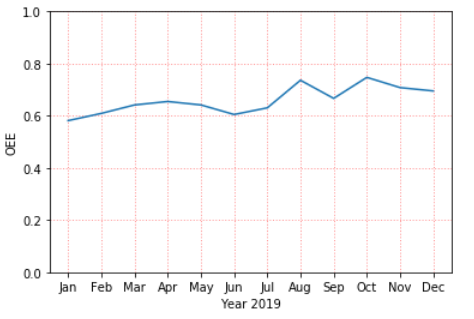
\includegraphics[width=3.3in]{photo/oee_last_year.png}
  %\vspace{-15pt}
  \caption{OEE change during last year}\label{OEELastYear}
  \end{center}
\end{figure}

Observing the  Fig.~\ref{OEELastYear} graph it highlights the fact that OEE has recorded a minimum during January and June also maximized in August and October. The typical question for this kind of scenario is why OEE has been changed so far. In order to identify the quantifiable reasons for the reduction of OEE, the following  Fig.~\ref{correlation} correlation matrix is generated between the factors that affect OEE. Without the implication of subjective reasons such as breakdowns has occurred, Start-up has been delayed for the reduction of OEE, by providing a correlation matrix, reasons can be provided in an accurate manner. Below is the correlation matrix for the year.\\


\begin{itemize}
  \item Pearson Correlation Coefficient 
\end{itemize}

Pearson’s correlation coefficient (Equ.~\ref{Pearson_Correlation}) is the test statistics that measures the statistical relationship, or association, between two continuous variables.  It is known as the best method of measuring the association between variables of interest because it is based on the method of covariance.  It gives information about the magnitude of the association, or correlation, as well as the direction of the relationship.

\begin{equation}\label{Pearson_Correlation}
r =
  \frac{ \sum_{i=1}^{n}(x_i-\bar{x})(y_i-\bar{y}) }{%
        \sqrt{\sum_{i=1}^{n}(x_i-\bar{x})^2}\sqrt{\sum_{i=1}^{n}(y_i-\bar{y})^2}}
\end{equation}

\begin{figure}[ht]
  \begin{center}
  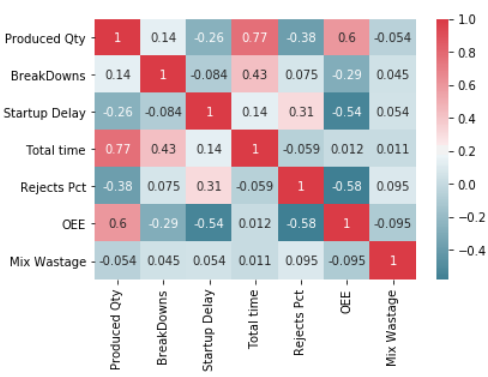
\includegraphics[width=3.3in]{photo/corr_all.png}
  %\vspace{-15pt}
  \caption{Correlation matrix against main attributes of the relation}\label{correlation}
  \end{center}
\end{figure}


By analyzing the correlation matrix it is highlighted that OEE has a strong positive correlation with Produced Quantity and Negative correlation with BreakDown Delays, Startup delays and Rejects percentage. Also, the Total time and the Mix wastage correlation can be negligible. To analyse the effects, the relevant correlated features were plotted with respect to the time. Fig.~\ref{comparison} shows the graph. 

\begin{figure}[ht]
  \begin{center}
  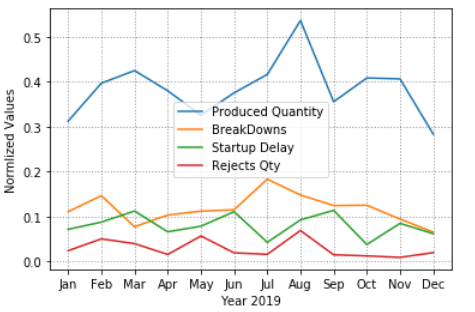
\includegraphics[width=3.3in]{photo/july_comp.png}
  %\vspace{-15pt}
  \caption{Month on Month variation on Produced Quantity Breakdowns Start-up Delay \& Rejects}\label{comparison}
  \end{center}
\end{figure}

On January Production Quantity is low and all other factors are average. Since the production quantity having a positive correlation with the OEE its obvious that that the OEE is reduced because of the quantity. July there is a huge increase in breakdowns the highest reported in 2019, which is highly negatively correlated with the OEE as the correlation graph shows. Its cleat that the increase in breakdowns brings the OEE down in July. 

When checking the August there is a huge increase in produced quantity so this is positively effected for the OEE to go up and on October the startup delay was minimum which results in a higher OEE on that month. \\

\subsection{Predictive Analysis}

This is the scenario where the output or the end result is being forecast based on the controllable or parameters that can be provided as targets. In this project, the focus will be to consider the set of parameters that are taken into consideration prior to planning a production run. Conventional production planning is carried out taken into consideration of two factors.

\begin{itemize}
  \item Demand for the period 
  \item Finished good stock level
\end{itemize}

Although this approach does the job of producing enough quantities for the period to satisfy the market demand, the efficiency factors are not considered in this process. Therefore this kind of planning might lead to in-efficient production runs. Therefore before starting manufacturing a product some targets have to be set. The following information was taken into consideration to predict whether a production run will be with acceptable OEE or not. By implementing this classifier, it enables to eliminate the unfavourable OEE thus making the plannings make sense in terms of profitability. \\

\begin{itemize}
  \item Product \\
  What are the products need to be manufactured: This is an input from the market condition and current stock levels: Macro Parameter
  \item Production Quantity \\
  How much products from each quantity should be produced: Also a macro factor which depends on the market conditions.
  \item Down Time \\
  Internal factor which can be assigned to a person as a target: This is the expected time that can be allowed for breakdowns.
  \item Start-up delay \\
  Internal factor which can be assigned to a person as a target. This is the expected maximum allowable time delay that can be there during the start-up process.
  \item Total Time \\
  Planned time to carry out the production-run: Internal parameter that is determined in planning stage.
  \item Rejects percentage \\
  Internal factor which can be assigned to a person as a target: This is the maximum allowable rejects(As a Percentage) that can happen during a production run. 
\end{itemize}

So for predictive analysis, the above variables were taken as features and the final prediction is the OEE. For these predictions, different methods were used. Following are the methods used and results obtained. \\
 \renewcommand{\labelitemi}{$\blacksquare$}
 
\subsubsection{Linear Regression}
The term “linearity” in algebra refers to a linear relationship between two or more variables. Linear regression performs the task to predict a dependent variable value (y) based on a given independent variable (x). So, this regression technique finds out a linear relationship between x (input) and y(output). Hence, the name is Linear Regression.

Linear regression was obtained for the selected feature set and tested for the test dataset. It achieved 86\% accuracy which is really good. \\


\subsubsection{Support Vector Machines}.
This supervised machine learning algorithm has strong regularization and can be leveraged both for classification or regression challenges. In the SVM algorithm, each data item is a point in n-dimensional space (where n is the number of features) with the value of each feature being the value of a particular coordinate. Then, perform classification by finding the hyper-plane that differentiates the two classes very well. In regression, Support Vector Machines algorithms use epsilon-insensitivity (margin of tolerance) loss function to solve regression problems.

The next approach was to use the Support Vector machines as a regressor for this problem. All these six features were selected and trained by this regressor. It gave 82.5\% accuracy for this. But this was lower than linear regression may be because SVM accuracy is lower for regression problems, unlike classification. \\


\subsubsection{Decision Trees}.
A decision tree is a decision support tool that uses a tree-like graph or model of decisions and their possible consequences, including chance event outcomes, resource costs, and utility. It is one way to display an algorithm that only contains conditional control statements.

Decision tree classifier was chosen to train the dataset initially. Sklearn library in python was used to train the regressor. It was given the accuracy of 76.03\% for the test dataset. 

Then hyperparameter tuning was used to further increase this value. Following parameters were obtained from the tuning


% =============== Table 1
\begin{center}
\begin{tabular}{ |l|c| } 
 \hline
 Matrix & Value  \\ 
 \hline
 Splitter & Best  \\
 Criterion & MAE  \\
 Min Samples split & 5  \\
 Min Samples leaf & 2  \\
 Max Features & None  \\
 Max Depth & 50  \\

 \hline
\end{tabular}
\end{center}

Using hyperparameter tuning, it was able to predict for the same dataset and reach 83.43\% of accuracy. Check the decision tree image using \href{https://github.com/DulanGit/In20-S1-CS5617-project-1/blob/master/output/Decision_Tree.png} {this link}. \\

\subsubsection{Random Forest Method}

Random forest, like its name implies, consists of a large number of individual decision trees that operate as an ensemble. Each individual tree in the random forest spits out a class prediction and the class with the most votes becomes our model’s prediction.

Then hyperparameter tuning was used to further increase this value. Following parameters were obtained from the tuning

\begin{center}
\begin{tabular}{ |l|c| } 
 \hline
 Matrix & Value  \\ 
 \hline
Num estimators & 800 \\
Criterion & MAE \\
Max features & auto \\
Max depth & 80 \\
Min samples split & 5  \\
Min samples leaf & 1 \\
 \hline
\end{tabular}
\end{center}
After hyperparameter tuning Random forest accuracy was improved from 88.27\% to  88.67\%. \\

\subsubsection{Deep Neural Networks}

A deep neural network (DNN) is an artificial neural network (ANN) with multiple layers between the input and output layers. The DNN finds the correct mathematical manipulation to turn the input into the output, whether it be a linear relationship or a non-linear relationship. Keras deep learning neural network \cite{Keras} library was used to create and train a neural network. Network architecture is shown in Fig.~\ref{deepneuralnetwork}

% ==== FIG 3
\begin{figure}[ht]
  \begin{center}
  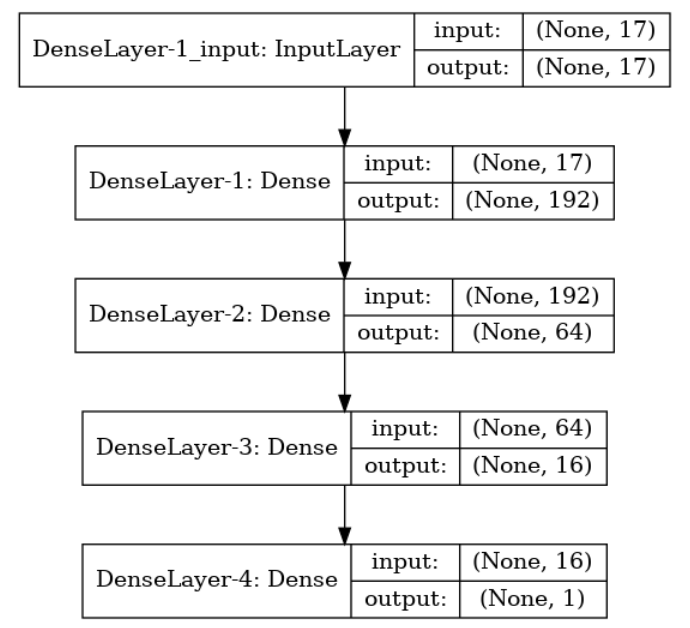
\includegraphics[width=2.5in]{photo/dnn.png}
  %\vspace{-15pt}
  \caption{Deep Neural Network Architecture}\label{deepneuralnetwork}
  \end{center}
\end{figure}

Hereafter several changes to the network architecture finally came up with this model which is not overfitting or underfitting. It gave a pretty good test accuracy for the current dataset after 100 epochs. The values after 100 epochs as below. 

% =============== Table 1
\begin{center}
\begin{tabular}{ |l|c| } 
 \hline
 Matrix & Value  \\ 
 \hline
 Training Loss & 0.0138  \\ 
 Validation Loss & 0.0344  \\ 
 Test Dataset accuracy & 93.04\%  \\ 
 \hline
\end{tabular}
\end{center}

Accuracies for all the above methods are summarized in the below table. 

\begin{center}
\begin{tabular}{ |l|c| } 
 \hline
Regression Method & Accuracy \\ 
 \hline\hline
Linear Regression & 84.48\% \\
Support Vector Machine & 80.43\% \\
Decision Tree & 83.43\% \\
Random Forest & 88.52\% \\
Neural Network & 94.21\% \\
 \hline
\end{tabular}
\end{center}

Different methods were taken to accurately predict the OEE with the available targets beforehand. Comparing the accuracy values for the above methods it's clear that the best accuracy was given by the NN model. It predicted the OEE with the accuracy of 94.21\% percent. 

These predictions are very valuable for a company like this. Starting a production line is a big task, its time and resource consuming. There is no easy way to make a decision when to start a new batch of products, most of the time with the experience one might take the decision based on that. With this approach, there is a clear prediction about how the outcome would be given the targets. Even a non-experienced person can now decide to start a new production line or not based on the information that is provided by these models.  

From these predictions, we are clear that we can predict the Overall Equipment Efficiency beforehand. This is very useful for the organization since it can foresee the outcome before even starting the production. 


\section{Conclusion}
The main objective of this project is to introduce Data-Driven Decision making for a manufacturing environment where more weight is imposed on the data analysis and visualization steps. Data Analysis has been carried out in a descriptive, diagnosis \&  predictive manner by providing different answers on the data set which is taken into consideration. For the sake of summarising the work only a few aspects, each analysis criteria is illustrated in this report. But there are other possibilities that same analysis methods can be implemented in order to get in-depth insights. 

%  \cite{krizhevsky2012imagenet,jain2000statistical,provost2013data}. 
%  \cite{pandas,Keras,seaborn,latex}. 

\section*{Acknowledgment}


%Dr. Reveryrand would like to acknowledge the funding by XLIM, Limoges, France. 
The  authors  would  like  to  thank  Dr. Uthayasanker Thayasivam and  Dr. A Shehan Perera  at University of Moratuwa for providing guidance to complete this project. 

% if have a single appendix:
%\appendix[Proof of the Zonklar Equations]
% or
%\appendix  % for no appendix heading
% do not use \section anymore after \appendix, only \section*
% is possibly needed

% use appendices with more than one appendix
% then use \section to start each appendix
% you must declare a \section before using any
% \subsection or using \label (\appendices by itself
% starts a section numbered zero.)
%

% ============================================
%\appendices
%\section{Proof of the First Zonklar Equation}
%Appendix one text goes here %\cite{Roberg2010}.

% you can choose not to have a title for an appendix
% if you want by leaving the argument blank
%\section{}
%Appendix two text goes here.


% use section* for acknowledgement
%\section*{Acknowledgment}


%The authors would like to thank D. Root for the loan of the SWAP. The SWAP that can ONLY be usefull in Boulder...


% Can use something like this to put references on a page
% by themselves when using endfloat and the captionsoff option.
\ifCLASSOPTIONcaptionsoff
  \newpage
\fi



% trigger a \newpage just before the given reference
% number - used to balance the columns on the last page
% adjust value as needed - may need to be readjusted if
% the document is modified later
%\IEEEtriggeratref{8}
% The "triggered" command can be changed if desired:
%\IEEEtriggercmd{\enlargethispage{-5in}}

% ====== REFERENCE SECTION

%\begin{thebibliography}{1}

% IEEEabrv,

\bibliographystyle{IEEEtran}
\bibliography{IEEEabrv,Bibliography}
%\end{thebibliography}
% biography section
% 
% If you have an EPS/PDF photo (graphicx package needed) extra braces are
% needed around the contents of the optional argument to biography to prevent
% the LaTeX parser from getting confused when it sees the complicated
% \includegraphics command within an optional argument. (You could create
% your own custom macro containing the \includegraphics command to make things
% simpler here.)
%\begin{biography}[{\includegraphics[width=1in,height=1.25in,clip,keepaspectratio]{mshell}}]{Michael Shell}
% or if you just want to reserve a space for a photo:

% ==== SWITCH OFF the BIO for submission
% ==== SWITCH OFF the BIO for submission
\begin{IEEEbiography}[{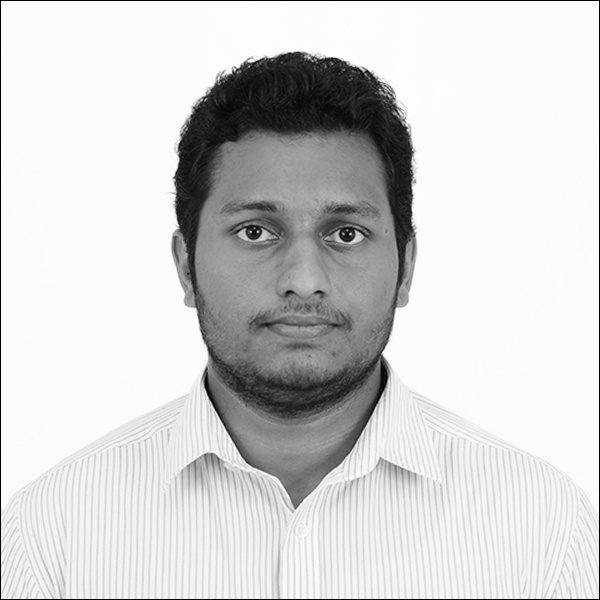
\includegraphics[width=1in,height=1.25in,clip,keepaspectratio]{photo/dulanjg.jpg}}]{Dulan Jayasuriya}
received the BSc in Engineering specialized in Electronic and Telecommunication Engineering from the University of Moratuwa in 2017, currently following an MSc program in Computer science in University of Moratuwa.
\end{IEEEbiography}
\begin{IEEEbiography}[{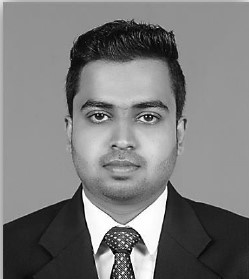
\includegraphics[width=1in,height=1.25in,clip,keepaspectratio]{photo/chanindug.jpg}}]{Chanindu Leelananda}
received the BSc in Engineering specialized in Electrical Engineering from the University of Moratuwa in 2017, currently following an MSc program in Computer science in University of Moratuwa.
\end{IEEEbiography}
%% if you will not have a photo at all:
%\begin{IEEEbiographynophoto}{Ignacio Ramos}
%(S'12) received the B.S. degree in electrical engineering from the University of Illinois at Chicago in 2009, and is currently working toward the Ph.D. degree at the University of Colorado at Boulder. From 2009 to 2011, he was with the Power and Electronic Systems Department at Raytheon IDS, Sudbury, MA. His research interests include high-efficiency microwave power amplifiers, microwave DC/DC converters, radar systems, and wireless power transmission.
%\end{IEEEbiographynophoto}

%% insert where needed to balance the two columns on the last page with
%% biographies
%%\newpage

%\begin{IEEEbiographynophoto}{Jane Doe}
%Biography text here.
%\end{IEEEbiographynophoto}
% ==== SWITCH OFF the BIO for submission
% ==== SWITCH OFF the BIO for submission



% You can push biographies down or up by placing
% a \vfill before or after them. The appropriate
% use of \vfill depends on what kind of text is
% on the last page and whether or not the columns
% are being equalized.

\vfill

% Can be used to pull up biographies so that the bottom of the last one
% is flush with the other column.
%\enlargethispage{-5in}



% that's all folks
\end{document}


